\section*{Chapter~5~~Evaluation}
\setcounter{section}{5} \setcounter{subsection}{0} 
\setcounter{table}{0} \setcounter{figure}{0} \setcounter{equation}{0}\setcounter{definition}{0}
\addcontentsline{toc}{section}{\textbf{Chapter~5~~Evaluation}}

% \subsection{Evaluation}

\subsection{Experiment Preparation}
\noindent This section describes the experimental framework used to evaluate the efficacy of the BLEGuard system. The settings are meticulously designed to mimic realistic scenarios in which BLE networks operate, ensuring that the results are both robust and applicable to real-world applications.



\subsubsection{Experimental Details}

\noindent The BLE-SAD dataset was compiled from nine distinct BLE devices, with their information detailed in \textbf{Appendices 1-1}. The dataset was divided into training and testing sets at a ratio of 8.5 to 1.5, comprising 762,850 effective BLE network packets for training and 134,088 for testing, respectively. The model training was conducted using an Intel Core i5-13600 CPU processor (3.50 GHz) with 32GB of RAM and an NVIDIA GeForce RTX 4060 Ti GPU equipped with 24GB of memory. The algorithms were implemented in Python 3.8, utilizing the PyTorch 1.8.1 framework.

\subsubsection{Parameter Settings}

\noindent In BLEGuard's Pre-detection Scheme, four crucial parameters (\(\Delta UCN_{\text{normal}}\), \(L_{\text{int}}\), \(\beta_{cfo}\), and \(\delta_{\text{rssi}}\)) are meticulously configured within specific ranges to maximize detection accuracy, as summarized in \textbf{Table 5-1}. These settings are the result of comprehensive testing and fine-tuning, ensuring that BLEGuard efficiently and reliably identifies spoofing attacks within BLE networks.

\begin{table}[h]
\renewcommand\arraystretch{1.32}
\centering
\caption{Optimal Parameter Settings for the Pre-detection Scheme.}
\begin{tabular}{l|l|l|l}
\bottomrule[0.64pt]
\textbf{Network Features} & \textbf{Parameter}         & \textbf{Setting Range} & \textbf{Optimal Setting} \\ \hline
Used Channel Numbers (UCN)                      & \(\Delta UCN_{\text{normal}}\) & (2.0, 5.0)                   & \textbf{2.8}                        \\
Advertising Interval (INT)                      & \(L_{\text{int}}\)            & (5.0, 20.0) ms          & \textbf{10.0 ms}                    \\
Carrier Frequency Offset (CFO)                      & \(\beta_{cfo}\)              & (1.0, 5.0)                   & \textbf{3.0}                        \\
Received Signal Strength Indicator (RSSI)                     & \(\delta_{\text{rssi}}\)     & (3.0, 10.0)                  & \textbf{5.0}                        \\ \toprule[0.64pt]
\end{tabular}
\end{table}

Additionally, \textbf{Table 5-2} provides a detailed account of the Temporal Convolutional Network's configuration, designed to process dynamic time-series data for immediate anomaly detection. \textbf{Table 5-3} expounds on the hyperparameters of the text-convolutional neural network model, employed to categorize packet data effectively into benign or malicious classes.


\begin{figure}%[H]
    \centering
    \caption*{Table 5-2 The hyperparameters of the temporal convolutional network network.}
    \vspace{-4pt}
    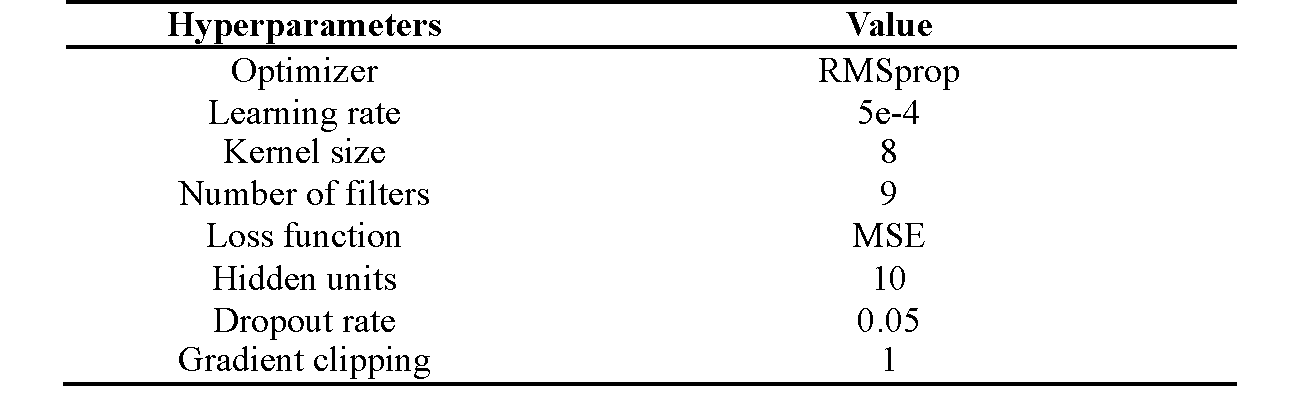
\includegraphics[width=0.95\linewidth]{FZU thesis templete//Table/table5-2.pdf}
\end{figure}


\begin{figure}%[H]
    \centering
    \caption*{Table 5-3 The hyperparameters of the text-convolutional neural network.}
    \vspace{-4pt}
    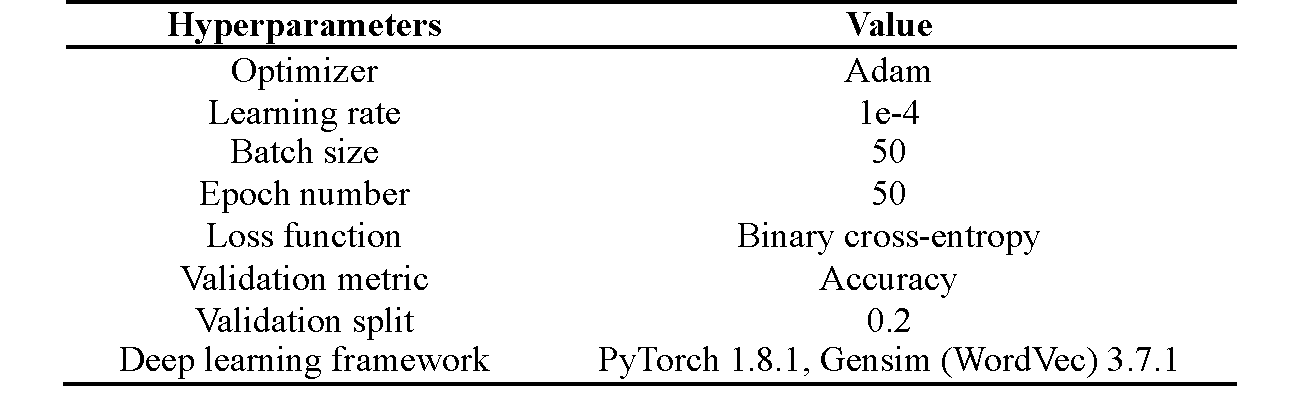
\includegraphics[width=0.95\linewidth]{FZU thesis templete//Table/table5-3.pdf}
\end{figure}




% ————————————————————————————————————————————————————————————————————— %
% ————————————————————————————————————————————————————————————————————— %


\subsection{Performance Evaluation Metrics}
\noindent In an effort to mirror a realistic network environment, the BLE-SAD dataset was intentionally constructed with an imbalanced proportion of benign to malicious packets. This imbalance, characterized by a predominance of benign samples, can induce skewed results. Consequently, the conventional metric of accuracy loses its representativeness and reliability as a sole measure of performance evaluation in such contexts. To mitigate the risk of biased analysis, more robust metrics like False Alarm Rate (FAR) and Un-detection Rate (UND) have been advocated for \cite{lahmadi2020mitm}. Therefore, in our performance evaluation, we extend beyond mere accuracy and incorporate FAR and UND. \textbf{Table 5-4} presents these evaluation metrics along with their respective formulas, defining TP, TN, FP, FN as follows:

\begin{itemize}[leftmargin=0.1cm]
    \setlength{\itemsep}{-0.1cm}
    \item TP (True Positive): Represents the number of malicious packets correctly classified as malicious.
    \item TN (True Negative): Represents the number of benign packets correctly identified as benign.
    \item FP (False Positive): Represents the number of benign packets incorrectly identified as malicious.
    \item FN (False Negative): Represents the number of malicious packets incorrectly identified as benign.
\end{itemize}


\begin{table}%[H]
    \tabcolsep=0.96cm
    \renewcommand\arraystretch{1.56}
    \centering
    \caption*{Table 5-4 Formula for three evaluation metrics}
    \vspace{-4pt}
    \begin{tabular}{cc}
    \toprule[1pt]
        % \specialrule{0em}{1pt}{1pt} 
        Evaluation metrics & Corresponding formula \\ \midrule[0.5pt]
        Accuracy & $\frac{T P+T N}{T P+T N+F P+F N} \times 100 \%$ \\
        False alarm rate (FAR) & $\frac{F P}{F P+T N} \times 100 \%$ \\
        Un-detection rate (UND) & $\frac{F N}{F N+T P} \times 100 \%$ \\
    \bottomrule[1pt]
    \end{tabular}
    \label{table5-4}
\end{table}


% ————————————————————————————————————————————————————————————————————— %
% ————————————————————————————————————————————————————————————————————— %


\subsection{Overall Performance Evaluation}

\noindent During the evaluation phase, three key metrics are employed to assess the effectiveness of our proposed methods. Accuracy, defined as the overall proportion of correctly classified instances, serves as a fundamental measure of the model's capability to accurately differentiate between benign and malicious packets. This metric is critical in evaluating the overall efficacy of the detection system. The False Alarm Rate (FAR) quantifies how often BLEGuard erroneously activates an alert when processing benign advertising packets from legitimate BLE devices, reflecting the model's precision. Conversely, the Un-detection Rate (UND) measures the frequency with which BLEGuard fails to identify a spoofing attack, highlighting potential vulnerabilities in detecting sophisticated threats.

\vspace{6pt}

BLEGuard's performance evaluation is conducted on a robust and imbalanced dataset collected from nine different BLE devices, such as Xiaomi sensors, Apple HomePod, and Dell speakers. The devices and the corresponding evaluation results are comprehensively detailed in \textbf{Table 5-5}. The table presents the performance metrics for each device, including the accuracy, FAR, and UND, thus providing a granular view of the system's effectiveness across varied hardware configurations. The empirical data from \textbf{Table 5-5} reveals BLEGuard's formidable detection capabilities, achieving an exemplary average accuracy of 99.02\%, complemented by a low false alarm rate of 2.04\% and an un-detection rate of 0.37\%. These statistics not only validate the robustness of BLEGuard but also illustrate its adaptability and reliability in diverse operational environments.

\vspace{4pt}

\begin{table}[H]
\centering
\tabcolsep=0.60cm
\renewcommand\arraystretch{1.16}
\caption*{Table 5-5 Detection performance of \textit{BLEGuard} mechanism.}
\vspace{-4pt}
% \resizebox{\textwidth}{!}{
\begin{tabular}{c|c|c|c|c}
\bottomrule[1pt]
\textbf{ID} & \textbf{Device (Number)}  & \textbf{Accuracy} & \textbf{FAR}  & \textbf{UND} \\ \hline \hline
 1 & Xiaomi Sensor (*3)     &   98.92\%         &    2.23\%         &    0.43\%         \\ \hline
 2 & Xiaomi Locker (*2)     &   99.11\%         &    2.04\%         &    0.32\%         \\ \hline
 3 & Xiaomi Speaker (*2)    &   98.93\%         &    1.84\%         &    0.36\%         \\ \hline
 4 & Apple HomePod (*1)     &   99.04\%         &    2.11\%         &    0.34\%         \\ \hline
 5 & Dell Speaker (*1)      &   99.21\%         &    2.51\%         &    0.17\%         \\ \hline
 6 & Lenovo Speaker (*1)    &   98.71\%         &    1.81\%         &    0.76\%         \\ \hline
 7 & August Smart Lock (*2) &   99.00\%         &    2.43\%         &    0.19\%         \\ \hline
 8 & Nutale Key Finder (*2) &   99.05\%         &    1.45\%         &    0.52\%         \\ \hline
 9 & Nordic nRF52 DK (*2)   &   99.20\%         &    1.96\%         &    0.22\%         \\ \hline \hline
\multicolumn{2}{c|}{\textbf{Overall}}   & \textbf{99.02\%}  &  \textbf{2.04\%}  & \textbf{0.37\%}   \\
\toprule[1pt]
\end{tabular}
% }
\end{table}

\noindent BLEGuard's performance, with a 2.04\% FAR and a 0.37\% UND, indicates high reliability for real-world BLE network monitoring. In a weeklong, intensive-use scenario, it would minimally misidentify benign activity or miss spoofing incidents, maintaining network integrity with little disruption. Such reliability translates into reduced maintenance demands and allows network administrators to focus their efforts on proactive improvements rather than reactive troubleshooting.


% ————————————————————————————————————————————————————————————————————— %
% ————————————————————————————————————————————————————————————————————— %


% \subsection{Classification Performance}

% \noindent As mentioned in \textbf{Section 4.3}, we utilized the text-CNN for features extraction, and evaluated the performances of five different classifiers (SVM, KNN, Random Forest, Logistic Regression and Naïve Bayes) in package classification. \textbf{Figure 5-1} depicts the accuracy performance for five machine learning classifiers. Within the training phase, the Random Forest (RF) model attains the highest accuracy at 99.41\%, whereas the SVM model exhibits the superior performance of 98.01\% in the testing results. In terms of the accuracy metric, the discrepancies between training and testing results are marginal, with one notable exception being the Logistic Regression (LR). This observation suggests that the LR classifier underperforms in realistic testing scenario. \\

% \begin{figure}[H]
%     \centering
%     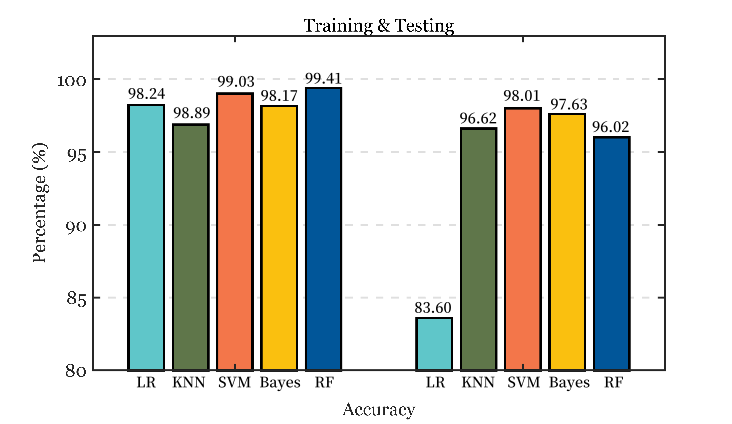
\includegraphics[width=0.8\linewidth]{FZU thesis templete//Fig/fig5-1.png}
%     \caption{The workflow of \textit{BLEGuard} detection mechanism.}
%     \label{fig-5-1}
% \end{figure}

% \noindent \textbf{Figure 5-2} provides a visual representation of the FAR comparison among five classifiers. In this context, FAR signifies the percentage of benign traffic incorrectly classified as malicious. Among these models, the Random Forest model exhibits the most favorable FAR of 0.01\% during the training experiments, while the SVM model outperforms others with a FAR of 0.09\% in the testing experiments. Nevertheless, when scrutinizing the variation between the training and testing scenarios, it becomes apparent that the Random Forest model experiences a relatively substantial increase, rising from its initial 0.01\% to 0.24\%. This upward shift suggests a potential instability in the model's performance when subjected to realistic testing conditions. Furthermore, the Logistic Regression model continues to exhibit suboptimal performance, registering the highest FAR of 2.47\% among all models, thereby establishing itself as the least performing model in this phase. \\

% \begin{figure}[H]
%     \centering
%     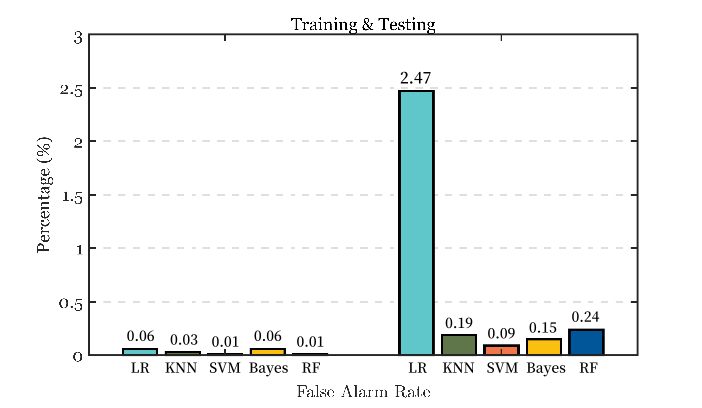
\includegraphics[width=0.8\linewidth]{FZU thesis templete//Fig/fig5-2.png}
%     \caption{The workflow of \textit{BLEGuard} detection mechanism.}
%     \label{fig-5-2}
% \end{figure}

% \noindent \textbf{Figure 5-3} presents the performance of UND for the five models. In this stage, UND denotes the percentage of malicious traffic inaccurately classified as benign traffic. Notably, the SVM model excels in this regard, achieving the lowest UND rate at 1.28\%. Following SVM, the Naïve Bayes (Bayes) model demonstrates a UND rate of 2.46\%, while the K-Nearest Neighbors (KNN) model and Random Forest (RF) model exhibit UND rates of 2.94\% and 3.71\%, respectively. Conversely, the LR model displays a notably poor performance, recording a high UND rate of 56.73\%. \\

% \begin{figure}[H]
%     \centering
%     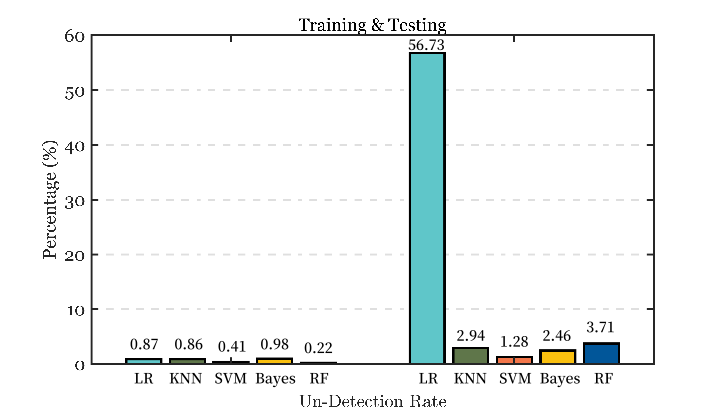
\includegraphics[width=0.8\linewidth]{FZU thesis templete//Fig/fig5-3.png}
%     \caption{The workflow of \textit{BLEGuard} detection mechanism.}
%     \label{fig-5-3}
% \end{figure}

% \noindent Overall, the preliminary results unequivocally highlight the outstanding performance of the Support Vector Machine (SVM) model, with the 98.01\% accuracy, 0.10\% FAR, and 0.81\% UND, as illustrated in \textbf{Table 5-2}.




% \subsection{Energy Overhead}



\newpage